
%(BEGIN_QUESTION)
% Copyright 2006, Tony R. Kuphaldt, released under the Creative Commons Attribution License (v 1.0)
% This means you may do almost anything with this work of mine, so long as you give me proper credit

Three pressure gauges (labeled {\bf A}, {\bf B}, and {\bf C}) are measuring water pressure at different points in a piping system:

$$\includegraphics[width=15.5cm]{i00707x01.eps}$$

An ultrasonic flowmeter clamped to the outside of the straight 2" pipe measures a flow velocity of 65 feet per second.  The pressure gauge at that point ({\bf B}) registers 22 PSI.  Pressure gauge {\bf A}, connected to the upper section of 8" pipe, is located 30 inches higher than pressure gauge {\bf B}.  Pressure gauge {\bf C} is located 22 inches lower than pressure gauge {\bf B}.  Assuming no energy lost due to friction, calculate the following:

\begin{itemize}
\item{} The water's velocity ($v$) in the 8" pipe near pressure gauge {\bf A} = \underbar{\hskip 50pt} ft/s
\vskip 5pt
\item{} The water pressure ($P$) registered by pressure gauge {\bf A} = \underbar{\hskip 50pt} PSI
\vskip 5pt
\item{} The water pressure ($P$) registered by pressure gauge {\bf C} = \underbar{\hskip 50pt} PSI
\vskip 5pt
\item{} The water flow rate ($Q$) in the 8" pipe near pressure gauge {\bf C} = \underbar{\hskip 50pt} GPM
\end{itemize}

\underbar{file i00707}
%(END_QUESTION)





%(BEGIN_ANSWER)

4 points for correct velocity in 8" pipe, 2 points each for all other answers:

\begin{itemize}
\item{} The water's velocity ($v$) in the 8" pipe near pressure gauge {\bf A} = \underbar{\bf 4.063} ft/s
\vskip 5pt
\item{} The water pressure registered by pressure gauge {\bf A} = \underbar{\bf 49.426} PSI
\vskip 5pt
\item{} The water pressure registered by pressure gauge {\bf C} = \underbar{\bf 51.304} PSI
\vskip 5pt
\item{} The water flow rate ($Q$) in the 8" pipe near pressure gauge {\bf C} = \underbar{\bf 636.48} GPM
\end{itemize}

%(END_ANSWER)





%(BEGIN_NOTES)

{\bf This question is intended for exams only and not worksheets!}.

%(END_NOTES)


